\documentclass[conference]{IEEEtran}
%\documentclass[english]{article}
%%%%%%%%%%%%%%%%%%%%%%%%%%%%%%%%%%%%%%%%%%%%%%%%%%%%%%%%%%%%%%%%%%%%%%%%%%%%%%%%%%%%%%%%%%%%%%%%%%%%%%%%%%%%%%%%%%%%%%%%%%%%
\usepackage{float}
\usepackage{graphicx}
\usepackage{amsmath}
\usepackage{comment}
\usepackage{caption}
\usepackage{subcaption}
\usepackage[latin9]{inputenc}
\usepackage[letterpaper]{geometry}
\geometry{verbose,tmargin=1in,bmargin=1in,lmargin=0.75in,rmargin=0.75in}
\usepackage{latexsym,amsmath,amssymb,amsfonts,fullpage}
\makeatletter
\renewcommand{\dddot}[1]{%
  {\mathop{\kern\z@#1}\limits^{\vbox to-1.4\ex@{\kern-\tw@\ex@
   \hbox{\normalfont ...}\vss}}}}
\renewcommand{\ddddot}[1]{%
  {\mathop{\kern\z@#1}\limits^{\vbox to-1.4\ex@{\kern-\tw@\ex@
   \hbox{\normalfont....}\vss}}}}
\makeatother
\newcommand{\argmin}{\arg\!\min}
\newcommand{\Lagr}{\mathcal{L}}
\setcounter{MaxMatrixCols}{20}

%\title{CIS 563 Final Project Report}
%\author{Samantha Cohen \\ Sarah Leung}
%\date{\vspace{-5ex}}
\title{Position-Based Fluid Simulation}
\author{\IEEEauthorblockA{Samantha Cohen} \and \IEEEauthorblockA{Sarah Leung}}

\begin{document}
\maketitle
\thispagestyle{plain}
\pagestyle{plain}

\section{Introduction}

For our final project, we chose to implement water simulation using position-based fluid dynamics. This is a method developed by Macklin and Muller [1] that is essentially a combination of traditional smoothed-particle hydrodynamics (SPH) and position-based dynamics (PBD), which solves the dynamics of a system through constraint projection. We saw this topic as an opportunity to expand on several previous projects, as well as implement additional features such as solid object interaction and rendering. 
\section{Overview of Position Based Fluids}
\subsection*{PBF vs. SPH}
The position-based fluids (PBF) method combines SPH [2], which is the traditional Lagrangian approach to simulating fluids, and position-based dynamics [3]. The dynamics of fluids are governed by two main laws of physics. The first is the Navier-Stokes equation: 
\begin{equation*}
\frac{\partial \bold u}{\partial t} + (\bold u \cdot \nabla) \bold u = -\frac{1}{\rho}\nabla p + \nu \Delta u + g
\end{equation*}
The second is the conservation of momentum: 
\begin{equation*}
\nabla \cdot \bold u = 0 
\end{equation*}
The Navier-Stokes equation relates the velocity $\bold u$, pressure $p$, density $\rho$, and viscosity $\nu$, in the dynamics of fluids. Particle methods for simulation solve the Navier-Stokes equations on particles of water, looking primarily at the pressure and viscosity terms to describe its motion. 

In SPH, a Lagrangian approach, each particle carries properties, such as mass, pressure, density, position, and velocity. Since position-based fluids builds on PBD, the base properties that each particle carries are mass, position, and velocity. In our datastructure, we also have each particle carrying its density, which is solved for in each step. 

Some of the advantages the position-based fluids method has over SPH is integration stability, which allows for larger time steps. Additionally, we are able to use a smaller smoothing radius for the density constraint, while SPH requires a large number of neighbors to prevent deficiencies in the simulation. Finally, SPH has been known to have issues of tensile instability. In PBF, we add an artificial pressure term for surface tension, which reduces particle clumping and provides, for example, a more visually realistic splashing effect. 
\subsection*{Position Update}
Position-based fluids primarily solves a density constraint, which enforces the incompressibility of water. The density constraint is a function of the particle $i$ and its neighbors. 
\begin{equation*} 
C_i(\bold p_1, \dots, \bold p_n) = \frac{\rho_i}{\rho_0} - 1
\end{equation*}
Here $\rho_0 = 1000$ $kg/m^3$ is the rest density of water and $\rho_i$ is the density at particle $i$ given by the SPH density estimator, where $m_j$ is the mass on particle $j$:
\begin{equation*} 
\rho_i = \sum_{j}{m_j W(\bold p_i-\bold p_j,h)}
\end{equation*} 
The simulation uses a Jacobi solver to determine the position update, as a result of the effect of the neighboring particles. This requires the calculation of the scaling factor, $\lambda$ and artificial pressure term, $s_{corr}$, for the overall position delta, $\Delta \bold p$.
\begin{equation*}
\lambda_i = -\frac{C_i(\bold p_1, \dots, \bold p_n)}{\sum_{k}{|\nabla_{\bold p_k}C_i|^2+\epsilon}}
\end{equation*}
\begin{equation*}
s_{corr} = -k\left(\frac{W(\bold p_i-\bold p_j, h)}{W(\Delta \bold q, h)}\right)^n
\end{equation*}
\begin{equation*}
\Delta \bold p_i = \frac{1}{\rho_0}\sum_{j}{(\lambda_i+\lambda_j+s_{corr})\nabla W(\bold p_i-\bold p_j, h)}
\end{equation*}
\subsection*{XSPH Viscosity}
PBF deviates from the SPH viscosity calculation by using and artificial XSPH viscosity. This is calculated as a velocity update, which is done as a post-processing step, after the Jacobi solver loop. 
\begin{equation*}
\bold v_i^{new} = \bold v_i+c\sum_j{(\bold v_j-\bold v_i)\cdot W(\bold p_i-\bold p_j, h)}
\end{equation*}
\subsection*{Kernel Functions}
SPH and PBF use kernel functions to evaluate some of the quantities. In general, the Poly6 kernel is used for the density and viscosity calculations, while the gradient quantities for pressure or position update are evaluated using the gradient of the Spiky kernel. These kernels are listed below. Here, $h$ is the neighborhood radius and $\bold r$ is typically the distance vector from the neighbor to the particle. 
\begin{equation*} 
W_{poly6}(\bold r, h) = \begin{cases}
\frac{315}{64\pi h^9}(h^2-|\bold r|^2)^3, & \text{if } 0 \leq |\bold r| \leq h \\
0, & \text{otherwise}
\end{cases}
\end{equation*}
\begin{equation*} 
\nabla W_{spiky}(\bold r, h) = \begin{cases}
\frac{45}{\pi h^6}(h-|\bold r|)^2 \frac{\bold r}{|\bold r|}, & \text{if } 0 \leq |\bold r| \leq h \\
\bold 0, & \text{otherwise}
\end{cases}
\end{equation*}
\section{Aspects of the Simulation}
\subsection*{Solver Loop} 
The simulation runs through a loop at each time step, $\Delta t$. The predicted positions are first updated using velocity change due to external forces, which in our simulation is only gravity. Next, neighbor search is performed on these predicted positions, and the neighbors of each particle are stored. The following step is the solver loop of the simulation, run for 5-10 iterations typically, to solve the density constraint and artificial pressure term to obtain the position update. As a post-process, we update velocity according to the XSPH viscosity term, and finally perform collision detection. The last step updates the current position to the predicted position. 
\subsection*{Spatial Hashing} 
Initially, we started with an $O(n^2)$ neighbor search. Then we implemented spatial hashing for neighbor search as an acceleration structure for the simulation. The grid is discretized into cells, with width $h$ equal to the neighborhood radius. At each time step, each particle's grid coordinates are determined and hashed to a scalar key as in the equations below, with neighborhood radius $h$, minimum grid cell coordinates $\bold g_{min}$, and grid dimensions $\bold g$. 
\begin{equation*}
(i,j,k) = \text{ceil}\left(\frac{\bold p-\bold g_{min}}{h} \right)-\bold 1
\end{equation*}
\begin{equation*}
\text{key}(i,j,k) = g_y g_z i + g_z j + k
\end{equation*}
The particle is then pushed into the vector mapped to the key. Neighbors for each particle are also determined at each time step, before the solver loop. We first determine the grid cell the particle belongs to and then consider the cell and its 26 neighboring cells. We check all particles in those 27 cells to see if they fall within the neighborhood radius.
\subsection*{Collision Detection} 
For collision detection, we implemented static collision detection with the bounds of the box. The predicted position is updated to the inner surface of the bounding box and the velocity is reflected with a coefficient of restitution. We also implemented collision detection with static object meshes, using a naive particle-triangle intersection test. This test is implemented by first performing a plane intersection test, and then evaluating the intersection point against the barycentric coordinates of the triangle. To make the mesh-intersection test slightly faster, we first perform an intersection test with the bounding box of the mesh. This optimizes the speed while most particles are far from the mesh, but once particles enter the box containing the mesh, they still need to be checked against all triangles of the mesh. 

In the paper, the algorithm calls for collision detection and resolution to be performed within the Jacobi solver loop. However, we found that we could not update the velocity as required within the loop. We therefore moved the collision response part outside of the solver loop, after the viscosity calculation. 
\subsection*{Rendering}
For rendering in the simulation, we used openGL to render particles as spheres of a set radius. For visual debugging purposes, we colored the spheres according to the absolute values of the components of velocity. We attempted to use level sets to extract the water surfaces to a mesh for rendering, but ultimately did not get this working. Instead, we modified a script [4] to export particle positions and we wrote a MEL script to import the positions into Maya for rendering. All rendering was done on the CPU. 
\section{Challenges} 
Some challenges we faced were with the basic dynamics of water using position-based fluids. It was difficult to simultaneously debug our code and tune parameters to achieve more realistic movement of water. Additionally, we had some struggles with collision detection, first with the bounding box, which was essential to be able to capture the motion of water in a contained environment. We had problems with unstable particles bouncing off the walls and gradually escaping the box. 

Our biggest challenge was probably the time. Our simulation does not run in real time. For 1000 particles and a time step of 0.01 seconds, each simulation step takes a little over 0.2 seconds. When we add more particles, and an object file to the scene, the simulation frame rate decreases even more. Spatial hashing was an attempt to speed up time, but the time decresase for 1000 to 8000 particles was minimal, probably due to the overhead time for setup. OpenGL rendering also contributed to the slow speed of the simulation, since we are rendering a sphere for each particle, which need to be updated at each time step. 

For rendering, we also tried to implement level sets, and briefly looked into marching cubes, but due to lack of time, were unable complete integration of a third-party code into our simulation. We therefore kept with using the spheres for water particles, but exported the positions to Maya for more aesthetic rendering. 

\begin{figure}[H]
\centering
\begin{subfigure}{0.475\textwidth}
  \centering
  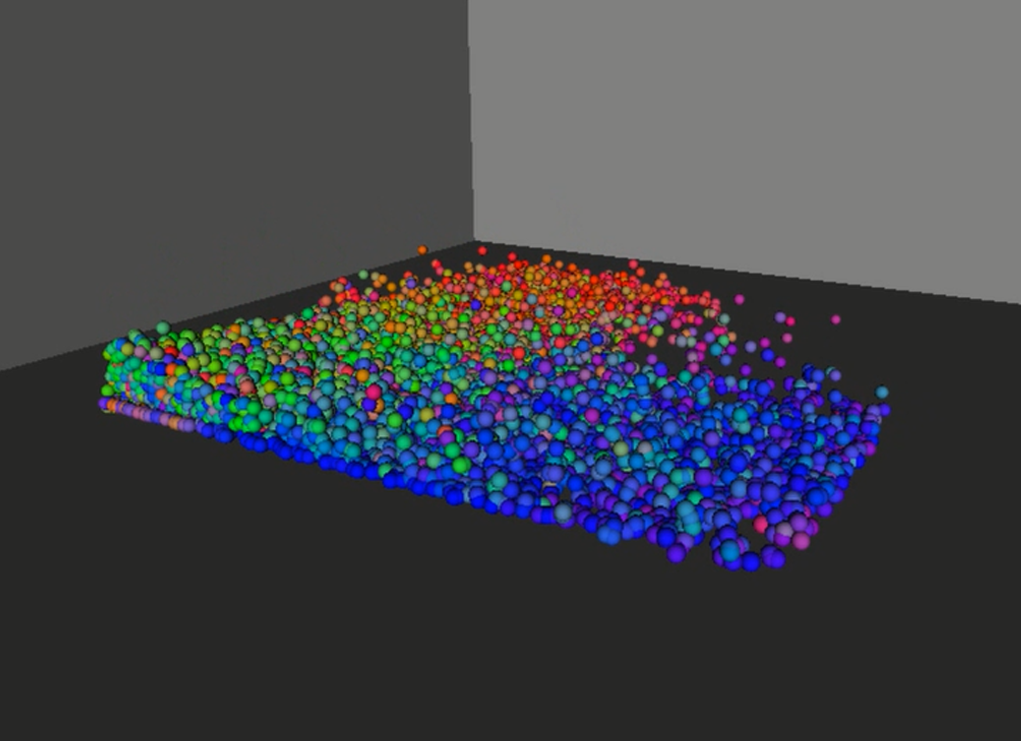
\includegraphics[width=1.0\linewidth]{without_scorr.png}
  \caption{Without the artificial pressure term, $s_{corr}$, there is particle clumping and overlapping.}
  \label{fig:without_scorr}
\end{subfigure}
\begin{subfigure}{0.475\textwidth}
  \centering
  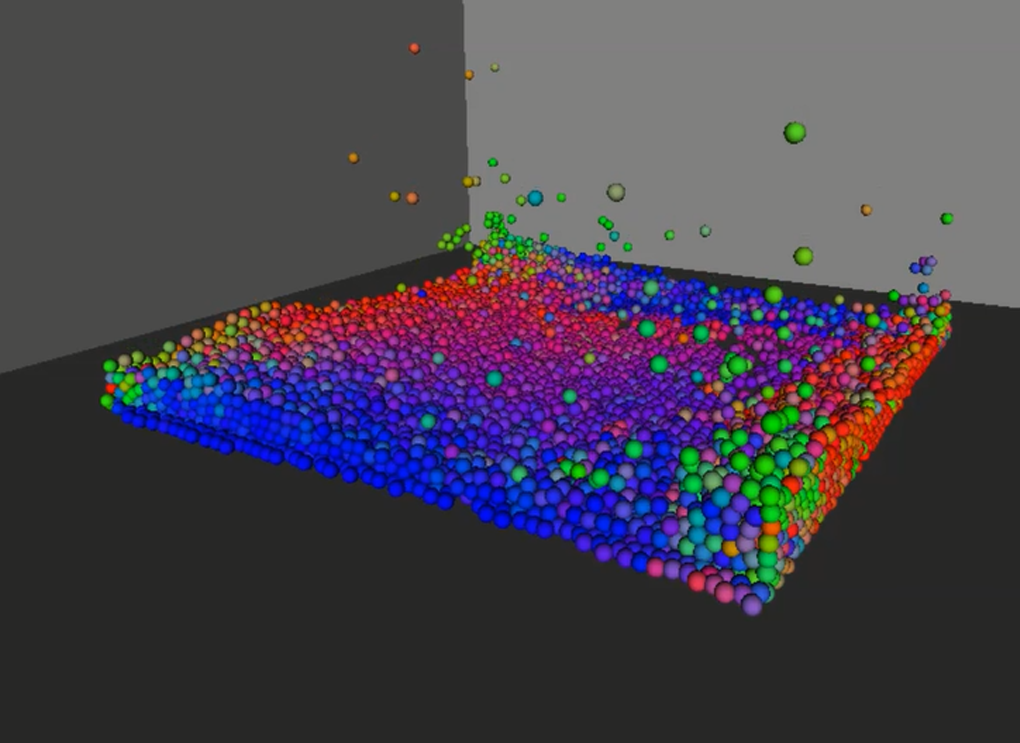
\includegraphics[width=1.0\linewidth]{with_scorr.png}
  \caption{With the addition of the artificial pressure term, $s_{corr}$, the particle distribution and surface tension is improved. }
  \label{fig:with_scorr}
\end{subfigure}
\caption{Artificial pressure term for tensile stability}
\label{fig:scorr}
\end{figure}
\section{Results}
The simulation achieves decent physically-based fluid motion for a smaller number of particles. We ran the simulation with the number of particles ranging from 1000 to 11375. The water was initiated as a uniform cube of particles, in the air, on the ground, or against a wall. We began with parameters suggested in the seminal paper, and tuned to stability and aesthetics. The neighborhood radius was one parameter that could be decreased to allow an increase in time optimality, while still retaining the motion of fluids. This is one advantage described in the paper that PBF has over SPH. Overall, the simulation is stables and provides fluid motion and splashing against walls. 

Figure 1 shows the difference in the simulation as a result of adding the artificial pressure term. Without the term, there is clumping of particles, and deficient particle distribution. When we add the artificial term, the particle distribution is vastly improved, such that the particles are compact without overlapping, providing the effect of surface tension. Figure 2 shows an example of water interacting with a fixed rigid object. It shows how the simulation can be used with particles of different radii, and handle collisions with medium-sized meshes. With smaller particles, there tends to be more instability, especially in collisions with object meshes. Figure 3 illustrates the effect of rendering the particles in Maya, creating a more visually appealing model of water. Figure 4 compares the openGL rendering with the Maya rendering for the case of water falling on a cow. 
\subsection*{Improvements and Future Work}
Some improvements that could me made are fine-tuning of parameters and collision detection for greater stability and time optimization to achieve real-time simulation. Future work could include rendering using level set or marching cube methods. 
\begin{figure}[H]
\centering
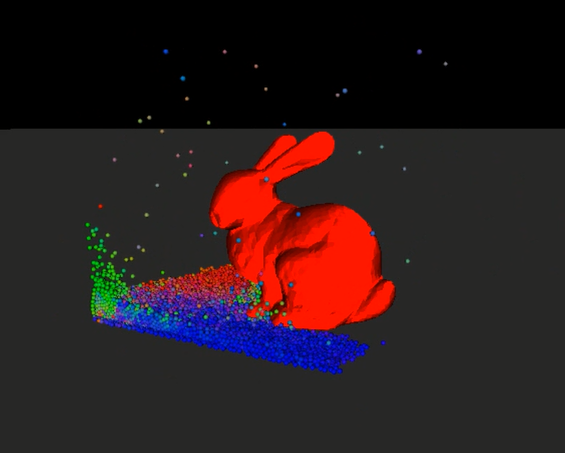
\includegraphics[width=1.0\linewidth]{bunny-1000-small.png}
\caption{Collision detection with object mesh, 8000 half-size particles}
\label{fig:collision_obj}
\end{figure}
\begin{figure}[H]
\centering
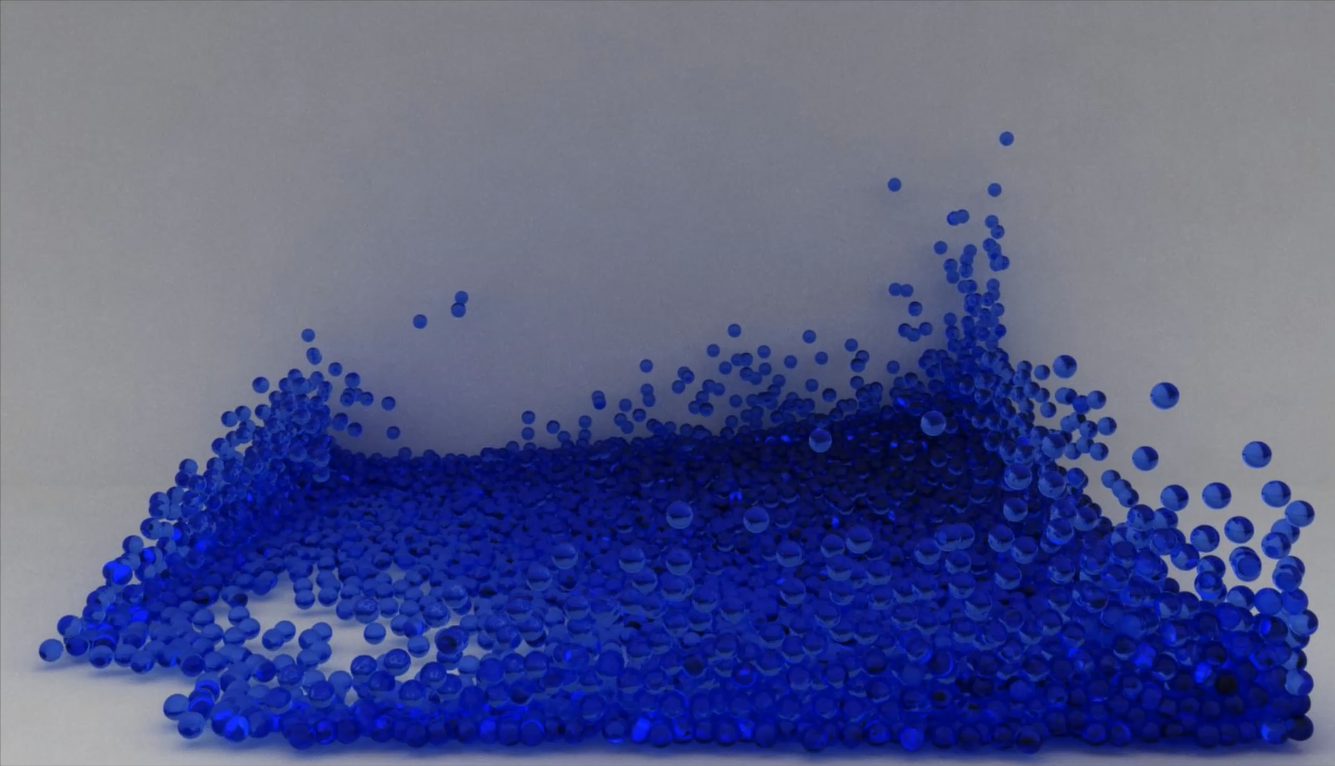
\includegraphics[width=1.0\linewidth]{compare_maya.png}
\caption{Maya rendering of spherical water particles}
\label{fig:maya_render}
\end{figure}
\begin{figure}[H]
\centering
\begin{subfigure}{0.475\textwidth}
  \centering
  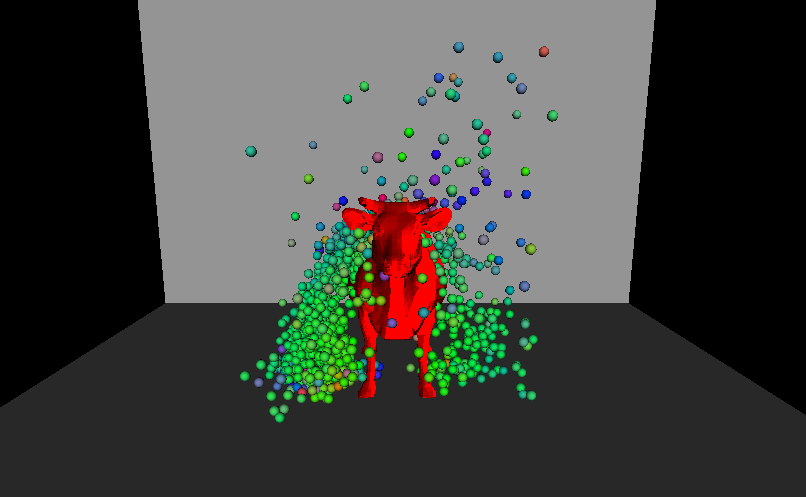
\includegraphics[width=1.0\linewidth]{WaterSimCow100.png}
  \caption{Water poured on a cow, openGL, 1000 particles}
  \label{fig:opengl_cow}
\end{subfigure}
\begin{subfigure}{0.475\textwidth}
  \centering
  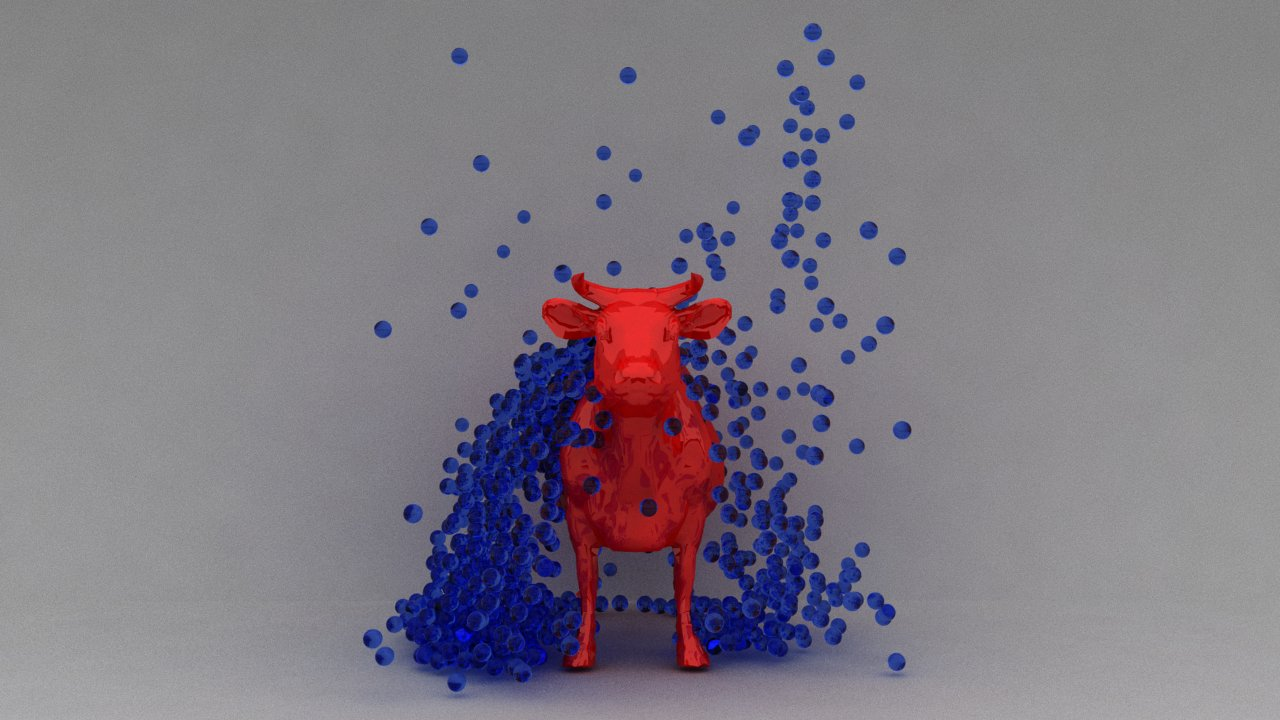
\includegraphics[width=1.0\linewidth]{WaterSimCow100-maya.jpg}
  \caption{Water poured on a cow, Maya, 1000 particles}
  \label{fig:maya_cow}
\end{subfigure}
\caption{Comparison of rendering methods}
\label{fig:render_compare}
\end{figure}
\section{Base Code} 
For this project, we used the completed ClothSim as our base code, as it uses position-based dynamics. This gave us a basic framework for setting up a position-based fluid simulation, since it is a position-based dynamics simulation to begin with. We used the basic datastructure for the storing of particles and their properties. We also used the main function, with modifications, to set up the simulation, with the water and environment. We worked off of the built-in openGL rendering scheme, adding a class to render the particles as spheres. Apart from this, all the math for fluid simulation, as well as the setup of the overall algorithm loop, collision detection, and object file loading were done on our own, without the use of third-party libraries. 

\section{Project Breakdown} 
Samantha worked on... 

Sarah worked on the position delta calculation, which included the density constraint, $\lambda$ for the constraint projection, and the artificial pressure term for tensile stability. She implemented the neighbor search and spatial hashing. She also worked on collision detection for the bounding box and object meshes. 


\bibliographystyle{IEEEtran}
\begin{thebibliography}{}

\bibitem{lamport94}
[Macklin $\&$ Muller 2013] Position Based Fluids. 

\bibitem{lamport94} 
[Muller et al. 2003] Particle-Based Fluid Simulation for Interactive Applications. 

\bibitem{lamport94}
[Muller et al. 2006] Position Based Dynamics. 

\bibitem{lamport94}
[Batty] https://raw.githubusercontent.com/christopherbatty/Fluid3D /master/main.cpp

\end{thebibliography}

\end{document}